\documentclass[UTF8]{ctexart}
\usepackage{graphicx}
\usepackage{listings}
\usepackage[colorlinks,linkcolor=red]{hyperref} %把颜色改成红色
\usepackage{xcolor}
\usepackage{amsmath}
\newtheorem{corollary}{Corollary}[section]
\usepackage{wrapfig}


\title{dfs序在图论问题的应用}
\author{赵涵铮}
\date{\today}	

\lstset{
	basicstyle          =   \sffamily,          % 基本代码风格
	keywordstyle        =   \bfseries,          % 关键字风格
	commentstyle        =   \rmfamily\itshape,  % 注释的风格,斜体
	stringstyle         =   \ttfamily,  % 字符串风格
	flexiblecolumns,                % 别问为什么,加上这个
	numbers             =   left,   % 行号的位置在左边
	showspaces          =   false,  % 是否显示空格,显示了有点乱,所以不现实了
	numberstyle         =   \zihao{-5}\ttfamily,    % 行号的样式,小五号,tt等宽字体
	showstringspaces    =   false,
	captionpos          =   t,      % 这段代码的名字所呈现的位置,t指的是top上面
	frame               =   lrtb,   % 显示边框
}

\lstdefinestyle{cpp}{
	language        =   C++, % 语言选Python
	basicstyle      =   \zihao{-5}\ttfamily,
	numberstyle     =   \zihao{-5}\ttfamily,
	breaklines      =   true,   % 自动换行,建议不要写太长的行
	columns         =   fixed,  % 如果不加这一句,字间距就不固定,很丑,必须加
	basewidth       =   0.5em,
}

\begin{document}
	\maketitle
	
	\section{异象石}
	\subsection{题目描述}
	给定有$n$个节点的树,$m$次操作,每次操作:
	\begin{enumerate}
		\item 选定一个点作为异象点
		\item 删除一个异象点
		\item 输出联通所有异象点的路径之和
	\end{enumerate}
	\subsection{数据范围}
	$1\leq N\leq 10^5,1\leq M\leq 10^5,1\leq X \leq Y\leq N$,数字不超过 C/C++ 的 int 范围	。
	\subsection{解题思路}
	根据题意,本题是对一棵树进行维护,由于树上两点只有唯一路径,所以是不需要考虑最短路径等问题的,只需要考虑如何维护临近的两点。
	
	我们可以先通过dfs,得到每一个点的时间戳,然后按照时间戳顺序,将异象点的节点排成首尾相连的一圈,累加两点之间的路径长度,最终得到的结果恰好是答案的两倍(每条边恰好经过两次)
	
	以此图为例,假设黑色的点为异象点:
	
	
		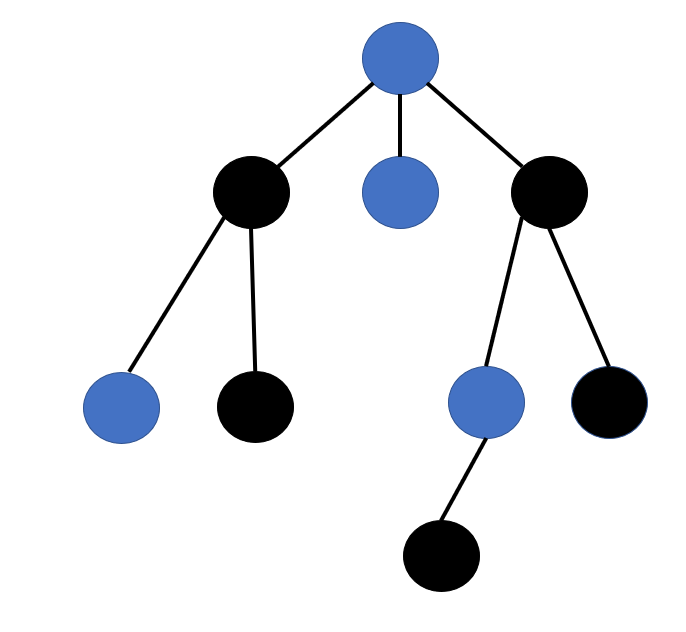
\includegraphics[width =0.3\linewidth]{./figure/simple}
	
	
	按照时间戳顺序,以此选择两个点,加粗表示两者路径,通过五次计算,加粗的边恰好被覆盖了两次:
	
		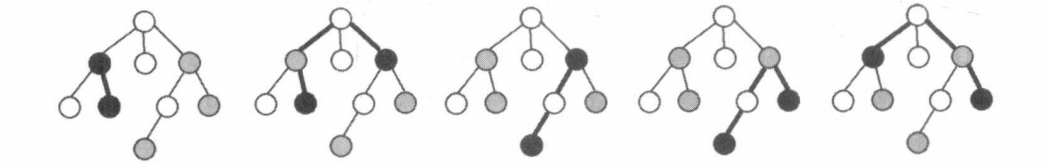
\includegraphics[width = \linewidth]{./figure/sum}
	
	为了维护好这个异象点集合,我们可以使用数据结构set,便于增删点,用ans来记录序列相邻点的路径长度之和(包括序列首尾)。
	
	接下来,我们需要解决如何计算任意两点距离的问题。设$path(x,y)$表示树上两点的路径长度,设$d[x]$表示$x$到根节点的路径长度,可知:
	\begin{equation}
		path(x,y)=d[x]+d[y]-2*d[LCA(x,y)]
	\end{equation}
	这样,就可以通过$LCA$算出$path(x,y)$,同时,我们可以通过一次$dfs$预处理好$d$数组。
	
	现在,让我们再次回顾一下全过程:若一个节点$x$出现了异象石,则根据时间戳,将节点$x$插入set中,它前后分别是$l$,$r$,则
	$$ans-path(l,r)+path(l,x)+path(x,r)$$
	若一个节点的异象点被删除,就类似的更新$set$。
	值得一提的是,$set$的插入和删除复杂度都是$O(\log N)$,时间复杂度为$O((N+M)\log N)$
	\subsection{参考代码}
%%	\lstinputlisting[
%	style       =   cpp,
%	caption     =   {异象石代码},
%	label       =   {problem1.cpp}
%%	]{problem1.cpp}
	
\end{document}